\documentclass[12pt, a4paper]{article}
\usepackage[utf8]{inputenc}
\usepackage[brazilian]{babel} % Hifenização e dicionário
\usepackage[left=3.00cm, right=2.00cm, top=3.00cm, bottom=2.00cm]{geometry}
\usepackage{enumitem} % Para itemsep etc
\usepackage{longtable} % Dependência do longtabu
\usepackage{tabu} % Para melhor criação de tabelas
\usepackage{color}
\usepackage{parskip} % Linha em branco entre parágrafos em vez de recuo
\usepackage{graphicx}
\usepackage[breaklinks]{hyperref}

\tabulinesep=0.75ex % Espaçamento interno das tabelas

\begin{document}

    \begin{titlepage}
        \flushright
        \rule{\textwidth}{1pt}
        {\large \textsc{UFRN --- Universidade Federal do Rio Grande do Norte
                \\[0.5ex]
         \normalsize DIMAp --- Departamento de Informática e Matemática Aplicada}
        \vspace{-0.5ex}}
        \rule{\textwidth}{1pt}

        \vfill

        {\Huge Sistema de Transparência Pública para a Assembleia Legislativa
        do RN \\[1ex] \LARGE Documento de Visão \\[2ex] \large Versão 2.0}

        \vfill

    \end{titlepage}

    \begin{tabu}{X | X[-1]}
        \hline
        Sistema de Transparência Pública para a Assembleia Legislativa do RN &
        UFRN
        \\ \hline

        Documento de Visão &
        Versão 2.0
        \\ \hline
    \end{tabu}

    \bigskip

    {\Large\textbf{Histórico de Revisão}}

    \vspace{2ex}

    \begin{tabu}{X[-1] | X[-1, r] | X | X[-1]}
        \hline
        \textbf{Data} &
        \textbf{Versão} &
        \textbf{Descrição} &
        \textbf{Autor}
        \\ \hline

        03/04/2014 &
        1.0 &
        Concepção do documento &
        Íslame Felipe
        \\ \hline

        05/04/2014 &
        1.1 &
        Leitura do documento com adição de informações e comentários &
        Felipe Cortez
        \\ \hline

        07/04/2014 &
        1.2 &
        Preenchimento inicial das tabelas de stakeholders e usuários,
        necessidades chave, perspectiva do produto e precedências e prioridades
        &
        Felipe Cortez
        \\ \hline

        07/04/2014 &
        1.3 &
        Formatação de capa e correção de erros &
        Felipe Cortez
        \\ \hline

        08/04/2014 &
        1.4 &
        Definições, acrônimos, abreviações, referências, requisitos e funcionalidades &
        Íslame Felipe
        \\ \hline

        08/04/2014 &
        1.5 &
        Formatação de capa, tabelas, correção de erros de digitação e edição de
        informações &
        Felipe Cortez
        \\ \hline

        08/04/2014 &
        1.6 &
        Acréscimo do diagrama de contexto, referências e restrições técnicas &
        Victor Almeida \newline Schinaider
        \\ \hline

        09/04/2014 &
        1.7 &
        Correções e revisão &
        Íslame Felipe
        \\ \hline

        09/04/2014 &
        1.8 &
        Mais correções e revisão &
        Felipe Cortez
        \\ \hline
        18/04/2014 &
        2.0 &
        Nova requisição: incluir o administrador do Sistema como stakeholder, bem como seus requisitos.   &
        Íslame Felipe
        \\ \hline
    \end{tabu}

    \newpage

    \tableofcontents

    \newpage

    \section{Introdução}
        \subsection{Finalidade}
        A finalidade deste documento é proporcionar uma perspectiva geral do
        projeto proposto, a fim de que seja possível compreender o seu produto.
        Assim, será possível entender as necessidades do sistema, as
        funcionalidades a serem implementadas e as restrições requisitadas.
        Este documento também visa entender o contexto da aplicação, seus
        stakeholders, requisitos, bem como desafios que devem ser enfrentados.

        \subsection{Escopo do documento}
        Este documento de visão se aplica ao Portal de Transparência da
        Assembleia Legislativa do Rio Grande do Norte. Este projeto propõe
        o desenvolvimento de um sistema web (na forma de portal) que deverá
        disponibilizar, de uma maneira transparente e imparcial, os aspectos
        que caracterizam os trâmites políticos, administrativos e econômicos da
        Assembleia Legislativa do Rio Grande do Norte.  Como exemplos de tais
        aspectos estão a atuação dos parlamentares nas sessões e nas votações
        de projetos importantes para a sociedade, bem como os projetos de leis
        que estão em votação atualmente. Eis o principal problema que deve ser
        resolvido: coletar informações concretas de tais aspectos e
        disponibilizá-las em um portal prático, isto é, de fácil manuseio e de
        pesquisa rápida, de modo a atrair o cidadão para que o mesmo possa
        usufruir do seu direito à informação.

        \begin{figure}[h]
            \centering
            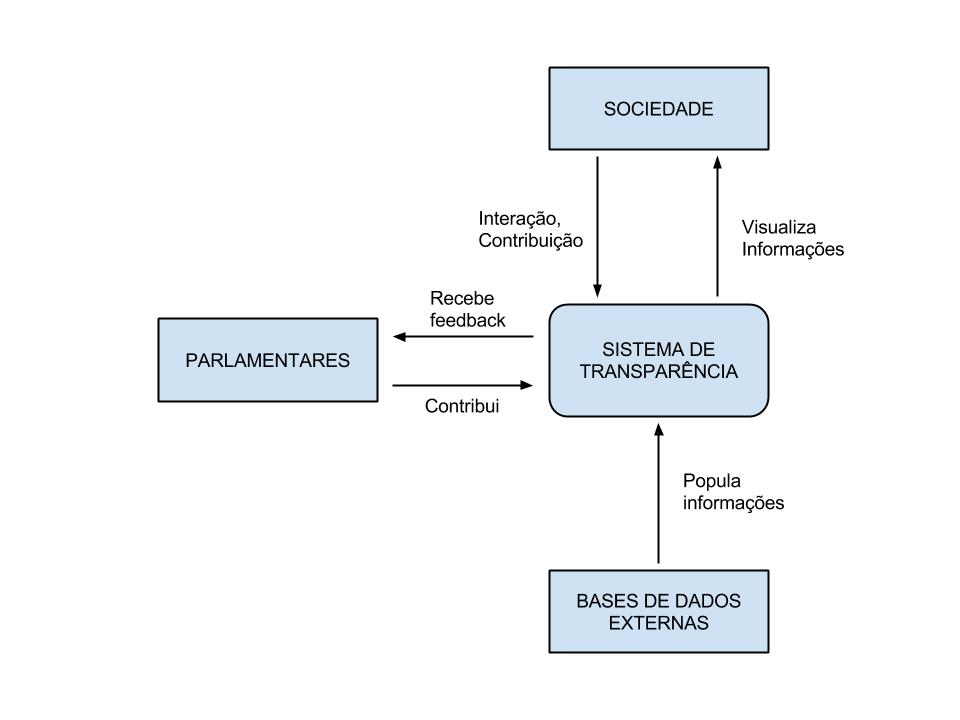
\includegraphics[width=15cm,height=11cm]{final.jpg}
            \caption{Diagrama de Contexto}
            \label{fig:mesh1}
        \end{figure}

        \subsection{Definições, acrônimos e abreviações}
            \begin{longtabu}{X[-1] | X}
                \hline
                \textbf{Palavra-chave} &
                \textbf{Definição}
                \\ \hline

                Parlamento &
                Constitucionalmente, e segundo o princípio da divisão dos
                poderes, constitui a sede do poder legislativo. Será
                representado pela Assembleia Legislativa do RN.
                \\ \hline

                Parlamentar &
                Indivíduo que compõe o parlamento. Pela Constituição vigente
                (de 1988), os parlamentares devem ser eleitos por eleições
                livres e diretas e têm a função de elaborar as leis de regem o
                Estado.
                \\ \hline

                Trâmites Legislativos &
                Termo de alto nível usado neste documento para referir-se a
                toda e qualquer atividade desempenhada no âmbito do poder
                legislativo, seja fora ou dentro de plenário. O termo abrange
                discussões e votações de projetos, liberações de verbas,
                debates em comissões, reuniões e etc.
                \\ \hline

                Projeto &
                Proposta, planejamento ou ideia que é escrita, analisada e
                votada em plenário, de acordo com o regimento interno da
                Assembleia e com a ordem de pautas. Pode referir-se a propostas
                de leis, de liberação de verbas, ou relacionado a assuntos de
                interesse geral da sociedade.
                \\ \hline

                Assessor &
                Indivíduo que presta serviço de assessoria individualmente ao
                parlamentar ou à Assembleia enquanto instituição.
                \\ \hline

                Sessão &
                Reunião ordinária ou extraordinária dos parlamentares no
                plenário da Assembleia. Nas sessões ordinárias, são debatidos
                assuntos importantes, analisados projetos ou realizadas
                votações. As sessões extraordinárias são solicitadas,
                geralmente, para homenagens, condecorações, ou votações
                urgentes. A presença em sessões é a atividade parlamentar mais
                básica.
                \\ \hline

                Comissões &
                Reuniões provisórias que congregam um subconjunto de
                parlamentares que devem analisar, investigar ou votar numa
                questão particular. A CPI (Comissão Parlamentar de Inquérito) é
                um exemplo de comissão que tem poder de investigação, a partir
                de escuta popular, de testemunhas ou de documentos.
                \\ \hline

                Orçamento público &
                É um instrumento de planejamento e execução das finanças
                públicas. Busca prever as despesas e receitas públicas. Deve
                ser votado pelo parlamento, portanto tem caráter de documento
                legal e é aprovado por lei.
                \\ \hline
            \end{longtabu}

        \subsection{Referências}
        \begin{itemize}
            \item
            \textbf{Site da Assembleia Legislativa -}
            \url{http://www.al.rn.gov.br/}
            \item
            \textbf{Regimento Interno da Assembleia Legislativa -}
            \url{http://www.al.rn.gov.br/portal/_ups/legislacao/regimentointerno.pdf}
            \item
            \textbf{Constituição do Estado do RN -}
            \url{http://www.al.rn.gov.br/portal/_ups/legislacao/constituicaoestadual.pdf}
            \item
            \textbf{Portal de transparência da AL -}
            \url{http://www.al.rn.gov.br/portal/transparencia/}
            \item
            \textbf{Portal de transparência do RS -}
            \url{http://www2.al.rs.gov.br/transparenciaalrs/PaginaInicial/tabid/2214/Default.aspx}
            \item
            \textbf{Portal de transparência de MG -}
            \url{http://www.almg.gov.br/sobre/transparencia/}
        \end{itemize}

    \section{Contextualização}
        \subsection{Descrição do problema}
            \begin{longtabu}{X[-1] | X}
                \hline

                \textbf{Problemas} &
                \begin{minipage}[t]{\linewidth}
                \begin{itemize}[itemsep=.5ex,parsep=.0ex,after=\strut,leftmargin=15pt]
                \item
                Poucas informações são divulgadas ao público. Dificuldade de
                acessar os dados apropriados.
                \item
                Os sistemas atuais não oferecem tanta facilidade de acesso à
                informação.
                \item
                Dificuldade de instigar o cidadão a fiscalizar os trâmites
                legislativos (o que lhe é de direito) através do uso da web.
                \end{itemize}
                \end{minipage}
                \\ \hline

                \textbf{Pessoas atingidas} &
                O cidadão é o principal agente atingido por este projeto, uma
                vez que o mesmo poderá inteirar-se acerca do que acontece na
                Assembleia, bem como das ações tomadas por parte dos seus
                representantes legislativos. A Assembleia Legislativa também
                deve ser beneficiada, pois terá a oportunidade de manter sua
                imagem transparente junto à população.
                \\ \hline

                \textbf{Cujo impacto é} &
                O principal impacto é o aprimoramento da visão crítica do
                cidadão, que poderá melhor discernir sobre suas próprias
                decisões no âmbito do seu exercício da democracia. A sociedade
                como um todo deve, portanto, ser beneficiada. A preocupação com
                a usabilidade facilitaria o acesso às informações.  Outro
                impacto, de certa forma, será a revelação de possíveis
                irregularidades que possam acontecer pelo mau uso do sistema
                representativo.
                \\ \hline

                \textbf{Uma solução \newline bem sucedida traria} &
                Uma solução ideal traria as informações mais relevantes à
                população, de modo claro, objetivo e imparcial. Pretendemos
                criar assim um portal de fácil manuseio e que coloca tais
                informações em primeiro plano.
                \\ \hline

            \end{longtabu}

        \subsection{Sentença de posição do produto}
            \begin{longtabu}{X[-1] | X}
                \hline
                \textbf{Para} &
                A sociedade em geral
                \\ \hline

                \textbf{Quem} &
                Por meio da equipe de desenvolvimento
                \\ \hline

                \textbf{O} &
                É um portal para a transparência da Assembleia Legislativa do RN
                \\ \hline

                \textbf{Que} &
                Proporcionar amplo acesso às informações acerca dos trâmites
                legislativos
                \\ \hline

                \textbf{Diferente de} &
                Portais de Transparência existentes que têm interface pouco
                amigável e pouco intuitiva
                \\ \hline

                \textbf{Nosso produto} &
                Traz a informação de maneira clara, objetiva e imparcial
                \\ \hline
            \end{longtabu}

    \section{Descrição dos stakeholders e dos usuários}
        \subsection{Principais stakeholders e usuários}

        \begin{longtabu}{X | X[2] | X[-1]}
                \hline
                \textbf{Identificação} &
                \textbf{Responsabilidades} &
                \textbf{Stakeholders}
                \\ \hline

                Gerentes do projeto &
                Gerenciar o acompanhamento do projeto. Avaliar a evolução do
                sistema. &
                Bernardo Gurgel
                \\ \hline

                Analistas de requisitos &
                Analisar os requisitos do sistema e do usuário. Realizar a
                verificação (corretude e coerência). Coordenar o processo de
                elicitação e especificação. &
                Íslame Felipe
                \\ \hline

                Arquiteto do projeto &
                Arquitetar o sistema. Propor a melhor forma de organizar as
                estruturas do sistema (modelo de arquitetura). &
                Felipe Cortez \newline
                Graco Babeuf \newline
                Íslame Felipe \newline
                Rubens Viana \newline
                Victor Schinaider
                \\ \hline

                Projetista de interfaces do projeto &
                Desenvolver e atualizar o projeto de interface de usuário,
                procurando deixá-la simples e intuitiva de acordo com os
                princípios de usabilidade. &
                Felipe Cortez
                \\ \hline

                Programadores &
                Desenvolver a codificação do sistema. Manter a integridade e
                evolução do código. Trabalho fundamentalmente em equipe. &
                Felipe Cortez \newline
                Graco Babeuf \newline
                Íslame Felipe \newline
                Rubens Viana \newline
                Victor Schinaider
                \\ \hline

                Organização &
                Prover a organização do projeto. &
                Ricardo Wagner \newline
                Rubens Viana \newline
                Victor Schinaider
                \\ \hline

                Usuário &
                Utilizar os incrementos do sistema. Emitir feedbacks sobre
                novos requisitos. &
                População geral
                \\ \hline
                
                Administrador do Sistema &
                Encarregado de administrar o portal e de atualizar o banco de dados do sistema. Deve ter acesso restrito a partir de login e senha.  &
                A ser designado pelo cliente.
                \\ \hline
            \end{longtabu}
            \newpage
        \subsection{Necessidades chave dos stakeholders e dos usuários}
            \begin{longtabu}{X[-1, r] | X | X[-1, r] | X[-1]}
                \hline
                \textbf{No.} &
                \textbf{Descrição} &
                \textbf{Prioridade \newline do cliente} &
                \textbf{Observações}
                \\ \hline

                1 &
                Conhecer os parlamentares, seus partidos, coligações e
                ideologias. Monitorar a atuação dos parlamentares e seu
                envolvimento nas atividades legislativas.
                & 1 &
                \\ \hline

                2 &
                Formar uma opinião pessoal acerca da atuação do parlamentar a
                fim de poder atuar da melhor maneira possível no processo
                eleitoral. &
                1 &
                \\ \hline
                3 &
                Conhecer os projetos eminentes, em pauta ou em espera pela
                pauta. Ter consciência da forma como os projetos são revertidos
                em benefícios à sociedade. &
                2 &
                \\ \hline
                4 &
                Conhecer o funcionamento da máquina pública. Poder acompanhar o
                direcionamento do dinheiro público. &
                2 &
                \\ \hline
                5 &
                Conhecer o funcionamento da Assembleia Legislativa do ponto de
                vista institucional. Aproximar-se do parlamento. &
                3 &
                \\ \hline
                 6 &
                Dispor de ferramentas e mecanismos capazes de auxiliar na atualização dos dados do portal.  Garantir acesso seguro à área restrita do site. &
                1 & Requisitos solicitado ao administrador do sistema na reunião do dia 14/04/2014.
                \\ \hline
            \end{longtabu}

    \section{Visão geral do produto}
        \subsection{Perspectiva do produto}

            \begin{longtabu}{X[-1, r]| X}
                \hline
                \textbf{Necessidades} &
                \textbf{Funcionalidades correspondentes}
                \\ \hline

                1 &
                Página detalhada do perfil do parlamentar
                \\ \hline

                1, 2 &
                Busca por sessões plenárias. Listar pauta, ata, resumo, data,
                parlamentares presentes e etc.
                \\ \hline

                3, 4 &
                Páginas que detalham comissões em andamento
                \\ \hline

                1, 2 &
                Página especial que associa o parlamentar a atividades
                desenvolvidas fora a assembleia.
                \\ \hline

                1, 2 &
                Mostrar detalhes de cada processo sofrido pelo parlamentar.
                \\ \hline

                1, 2 &
                Pesquisa histórico de processos do parlamentar.
                \\ \hline

                1, 2, 4, 5 &
                Listar a prestação de conta mensal da assembleia.
                \\ \hline

                1, 2, 4 &
                Página que detalha o gasto mensal do parlamentar
                \\ \hline

                1, 2 &
                Seção especial para a prestação de contas do parlamentar à
                justiça eleitoral
                \\ \hline

                2, 3, 4, 5 &
                Página que detalha as informações do orçamento público
                \\ \hline

                2, 3, 4, 5 &
                Download do texto na íntegra do projeto do orçamento
                \\ \hline

                3, 4 &
                Pesquisar projetos por categoria/natureza, por data, por status
                ou tema.
                \\ \hline

                3, 4 &
                Página que detalha projetos.
                \\ \hline

                2, 3, 4 &
                Página que noticia comissões, sessões, reuniões e outros assuntos.
                \\ \hline

                1, 2 &
                Pesquisar histórico de ex-parlamentar
                \\ \hline

                1, 2 &
                Página de contato do cidadão com o cliente
                \\ \hline
                 6  &
                Página de login para o administrador do sistema.
                
                \\ \hline
                6  &
                Página de Administração do Sistema. Tela de gerenciamento e que prover mecanismos e cadastro, edição e exclusão e informações (parlamentares, seções, projetos, comissões, gastos e etc.)
                
                \\ \hline
            \end{longtabu}

        \subsection{Premissas e dependências}
        O sistema é um portal web. Inicialmente deve-se desenvolvê-lo para
        acesso em qualquer navegador de um computador ligado à Internet.
        Posteriormente, pode-se pensar em abranger esta ideia para dispositivos
        móveis, ou até mesmo uma aplicação móvel. Uma dependência forte do
        sistema refere-se à sua alimentação. De fato, as informações devem, de
        alguma fonte (confiável), chegar a base dados do sistema. Assim,
        pode-se apresentar dependências de outras bases de dados que estejam em
        funcionamento com tais informações ou dependência direta de dados
        oriundos diretamente da Assembleia.

        \subsection{Limites do produto}
        O portal deve atender à legislação vigente quanto à divulgação de
        informações na Internet. Este projeto propõe uma fiscalização às
        atividades na Assembleia Legislativa, que envolve pessoas, como os
        parlamentares, assessores e secretários. As publicações no portal,
        inevitavelmente, devem envolver tais atores, desde que os mesmos
        participem de alguma atividade caracterizada por seu aspecto público ou
        que envolva, de algum modo, o uso de recursos públicos. Não serão
        publicadas, portanto, informações de cunho estritamente pessoal.

    \section{Requisitos funcionais do produto}
    \begin{itemize}
        \item
        Ter uma página com o perfil de cada parlamentar: considera-se este
        requisito como um dos mais básicos, uma vez que o usuário deverá ter
        conhecimento sobre cada um dos seus representantes, seus partidos e
        ideologias;
        \item
        Mostrar o envolvimento de cada parlamentar em atividades relacionadas
        ao uso do poder legislativo, como em votações, sessões, comissões,
        debates e etc
        \item
        Estender o requisito anterior para atividades fora da Assembleia, como
        a participação do parlamentar em causas e ações sociais
        \item
        Visualizar, detalhadamente, os processos sofridos por cada parlamentar.
        A ideia é emitir uma ficha que indique o quão “limpa” é a carreira
        política do deputado.
        \item
        Transparecer os gastos com o dinheiro público. Servirá como uma
        prestação de contas públicas que será disponibilizada ao cidadão.
        Atualmente, alguns sites já fazem isso, porém de maneira obscura. A
        ideia é que os gastos possam ser monitorados e atualizados em períodos
        regulares (como semanalmente ou mensalmente). Eles podem envolver cada
        parlamentar individualmente, através do uso de verbas de custeio ou
        para emendas parlamentares ou podem envolver a Assembleia enquanto
        instituição, por exemplo, seus gastos com pagamento de assessores,
        secretários, serviços, compras e licitações.
        \item
        Os gastos de cada parlamentar em campanhas eleitorais também devem ser
        monitorados. De fato, esta é uma atividade que tem a ver com a
        Assembleia Legislativa, pois apenas serão disponibilizados dados
        referentes a deputados eleitos pelo voto direto (e que, portanto, estão
        em exercício do poder legislativo), e que foram declarados à Justiça
        Eleitoral no momento do registro da candidatura.
        \item
        Os dados referentes ao orçamento público devem ter sua devida atenção.
        Uma vez que a proposta foi aprovada em plenário, o texto deve ser
        publicado na íntegra. Outra sessão deve ser criada para destacar as
        principais cláusulas do documento, como o valor total do orçamento,
        destino das verbas e previsões.
        \item
        Monitorar os projetos dos parlamentares (das mais diversas naturezas)
        que estão atualmente em discussão, os que foram aprovados ou
        reprovados, e os que estão em espera pela pauta. Criar infográficos
        interativos que separe bem estas categorias, evidenciando a importância
        da cada usa. Este requisito é importante pois o cidadão terá como
        conhecer as ideias do parlamento e poderá formar suas opiniões.
        \item
        Dedicar uma seção para aqueles projetos que foram votados e aprovados,
        mas que nunca saíram do papel. Apresentar o usuário uma satisfação
        sobre o ocorrido.
        \item
        Noticiar sessões, eventos, congressos e comissões que venham debater
        assuntos relevantes e de interesse geral da população.
        \item
        Possibilitar pesquisas rápidas em históricos, dos períodos legislativos
        passados. Manter uma base de dados para este requisito.
        \item
        Possibilitar do contato direto o cidadão com o parlamentar, através do
        envio de e-mail.
        \item
        Ferramentas de administração. O Administrador do Sistema poderá fazer login e, assim, poderá editar o banco de dados do portal, numa interface diretamente WEB. Para tanto, agirá sobre os dados: Parlamentar/Mandatos, Seção, Comissão, Processo, Projeto e Gastos. 
    \end{itemize}

    \section{Precedência e prioridades}

    \begin{longtabu}{X[-1, r] | X | X[-1, r] | X[-1]}
            \hline
            \textbf{No.} &
            \textbf{Funcionalidade} &
            \textbf{Prioridade \newline do cliente} &
            \textbf{Entrega}
            \\ \hline

            1 &
            Tela de login e subsistema de administração (cadastro, edição e exclusão). 
            & 1 & 22/04/2014
            \\ \hline
            
            2 &
            Página detalhada do perfil do parlamentar. &
            1 & 22/04/2014
            \\ \hline

            3 &
            Busca por sessões de plenárias. Listar pauta, ata, resumo, data,
            parlamentares presentes e etc. &
            2 & 29/04/2014
            \\ \hline

            4 &
            Mostrar detalhes de cada processo sofrido pelo parlamentar. &
            2 & 29/04/2014
            \\ \hline

            5 &
            Páginas que detalham comissões em andamento. &
            2 & 29/04/2014
            \\ \hline

            6 &
            Página que detalha o gasto mensal do parlamentar.
            & 2 & 29/04/2014
            \\ \hline

            7 &
            Seção especial para a prestação de contas do parlamentar à justiça
            eleitoral. &
            2 & 06/05/2014
            \\ \hline

            8  &
            Pesquisar projetos por categoria/natureza, por data, por status ou
            tema. &
            2 & 06/05/2014
            \\ \hline

            9  &
            Página que detalha projetos. &
            2 & 06/05/2014
            \\ \hline

            10  &
            Página especial que associa o parlamentar a atividades
            desenvolvidas fora a assembleia. &
            3 & 06/05/2014
            \\ \hline

            11 &
            Pesquisa histórico de processos do parlamentar. &
            3 & 13/05/2014
            \\ \hline

            12 &
            Listar a prestação de conta mensal da assembleia &
            3 & 13/05/2014
            \\ \hline

            13 &
            Página que detalha as informações do orçamento público &
            3 & 13/05/2014
            \\ \hline

            14 &
            Download do texto na íntegra do projeto do orçamento &
            4 & 13/05/2014
            \\ \hline

            15 &
            Página que noticia comissões, sessões, reuniões e outros assuntos.
            &
            4 & 20/05/2014
            \\ \hline

            16 &
            Pesquisar histórico de ex-parlamentar &
            4 & 20/05/2014
            \\ \hline

            17 &
            Página de contato do cidadão com o parlamentar &
            4 & 20/05/2014
            \\ \hline
            
            
        \end{longtabu}

    \section{Requisitos não-funcionais do produto}
    \begin{itemize}
        \item
        Requisitos de usabilidade: o portal deve apresentar uma interface
        amigável interativa, a fim de proporcionar ao usuário uma fácil
        navegação e compreensão do conteúdo exposto.
        \item
        O termo transparência deve ser convertido em um requisito
        não-funcional. Este é o diferencial do projeto proposto. De fato, deve
        ser fácil de se encontrar a informação, sem caminhos excessivamente
        longos que possam desencorajar o usuário de procurar pela informação.
        \item
        Toda publicação deve atender à legislação vigente. Além disso, deve ser
        feita de maneira imparcial, isto é, sem beneficiar nenhum partido
        político ou qualquer entidade.
        \item
        Deve-se assegurar a veracidade das informações.
    \end{itemize}

    \section{Restrições técnicas}
    \begin{itemize}
        \item
        O servidor que armazenará o sistema deve suportar uma carga alta de
        usuários simultâneos
        % Os itens seguintes são restrições técnicas?
        \item
        O sistema vai utilizar a ferramenta livre Play Framework
        \item
        Não teremos nenhum orçamento para realização do projeto
        \item
        O sistema precisa ser entregue próximo ao final da primeira quinzena de
        junho de 2014
    \end{itemize}

\end{document}

